\section{Framework Overview} \label{overview}
In this section, we propose our novel fully homomorphic database framework, 
called \NAME,
to query and process encrypted data with high security, cost-effectiveness
and ease of outsourcing. We briefly review the overall architecture
and then provide a straightforward example to illustrate the \NAME workflow.
Meanwhile, we analyze the threat model and security guarantees of \NAME.

\subsection{\NAME Workflow} \label{overview:workflow}
\cref{fig:overview} outlines the framework architecture the \NAME 
with an intuitive example, where a user outsourced her daily health 
monitor data like heart rate (HR) as well as blood pressure (BP) 
and is interested in the prediction of heart disease. 
A high-level overview of
\NAME’s workflow (as shown in \cref{fig:overview}) is as follows:

\begin{figure*}[t!]
    % \[ % start math mode, center the contents
    \begin{tabular}{lp{6cm}<{\raggedright }cp{6.5cm}<{\raggedright }}
    \toprule
    & Client & & Server \\
    \midrule
    \multicolumn{2}{l}{Offline} & & \\
    1.& Set up FHE parameters: $Init(\lambda)$ & & \\
    2.& Init Table $\mathcal{T} = (t_1, t_2, ..., t_{\lvert \mathcal{T} \rvert_c})$ & &\\
    3.& Data Encryption: $\mathcal{CT} = \texttt{TableEnc}(\mathcal{T}) = 
    (ct_1, ct_2, ..., ct_{\lvert \mathcal{T} \rvert_c})$ & 
    $\xrightarrow{\quad\mathcal{CT}\quad}$ & Encrypted Table: $\mathcal{CT}$ \\
    \midrule
    \multicolumn{2}{l}{Online} & & \\
    4.& Init Query: $\mathcal{Q} = (p_{1}, p_{2}, ..., p_{\lvert \mathcal{Q} \rvert_p}, \mathcal{B}, \mathcal{F}, \mathcal{A})$ & & \\
    5.& Query Encryption: $\mathcal{CQ} = \texttt{QueryEnc}(\mathcal{Q})= 
    (cp_{1}, cp_{2}, ..., cp_{\lvert \mathcal{Q} \rvert_p}, \mathcal{B}, \mathcal{F}, \mathcal{A})$ & 
    $\xrightarrow{\quad\mathcal{CQ}\quad}$ & Encrypted Query: $\mathcal{CQ}$ \\
    7.& & & Query Evaluation: $ \mathcal{CR}_{\mathcal{Q}} = \texttt{QueryEva}(\mathcal{CT}, \mathcal{CQ}) = (cr_1, cr_2,..., cr_{\lvert \mathcal{A} \rvert})$ \\
    8.& Init Model: $\mathcal{M} = (m_{1}, m_{2}, ..., m_{\lvert \mathcal{M} \rvert_c}, 
    \mathcal{C})$ & & \\
    9.& Model Encryption: $\mathcal{CM} = \texttt{ModelEnc}(\mathcal{M})
    = (cm_1, cm_2, ...,cm_{\lvert \mathcal{M} \rvert_c}, \mathcal{C})$ &
    $\xrightarrow{\quad\mathcal{CM}\quad}$ & Encrypted Model: $\mathcal{CM}$ \\
    10.& & & Model Evaluation: $ \mathcal{CR}_{\mathcal{M}} = \texttt{ModelEva}(\mathcal{CM}, \mathcal{CR}_{\mathcal{Q}})$ \\
    11.& Result Decryption: $\mathcal{R} = \texttt{Decrypt}(\mathcal{CR})$ & 
    $\xleftarrow{\quad\mathcal{CR}\quad}$ & Evaluation Result:  $\mathcal{CR}_{\mathcal{M}}$\\
    \bottomrule
    \end{tabular}
    % \]
\caption{Kamto \dots}
\end{figure*}

\textbf{\textcircled{1} Line 1-3, Data Encryption }: In client side, the user first 
need to encrypt her data     using FHE schemes before uploading her data to 
the cloud server. 
As sketched in \cref{fig:overview}, Alice outsources her health data 
to a cloud server, 
she collects her daily health data 
in table \texttt{health} and encrypts the tangible value of rows 
in \texttt{health} under her secret key.
\begin{algorithm}[htbp]
    % \tiny
    \caption{Homomorphic Table Encryption Algorithm}
    \label{algo: query_evaluation}
    \SetKwInOut{Input}{Input}\SetKwInOut{Output}{Output}\SetKwInOut{Return}{Return}
    \Input{Ecrypted table $\mathcal{T}=
    (ct_{1}, ct_{2}, ... , ct_{\lvert \mathcal{T} \rvert_{c}})$\\
    Encrypted Query $\mathcal{Q}=
    (cp_{1}, cp_{2}, ... ,cp_{\lvert \mathcal{Q} \rvert_{p}}, \mathcal{B}, \mathcal{F}, \mathbf{A})$, where $G = (g_1, g_2, ..., g_{\lvert \mathcal{Q} \rvert_{p} - 1}, F = (f_1, ..., f_{\lvert \mathcal{Q} \rvert_{g}}$}
    \Output{A LWE ciphertext $ct_{O} = {\rm LWE}_{n,q}({\rm MSB}(m))$.}
    
    \Return{$ct_{O} = (b' + \mu, \mathbf{a}) 
    = {\rm LWE}_{n,q}({\rm MSB}(m))$}
\end{algorithm}

\textbf{\textcircled{2} Line 4-5, Query Encryption}: The cloud server stores 
user's encrypted records and could not gain any information without 
the secret key of the user. 
While the user is willing to query her data, 
she needs to encrypt the sensitive part of the query. 
As depicted  in \cref{fig:overview}, 
Alice wants to query the average value of HR and BP in the last month,
she encrypts the attribute fields in SQL queries and sents the 
encrypted query to the cloud server.

\textbf{\textcircled{3} Line 7, Query Processing}: Based on the user's encrypted query, 
the cloud server processes the encrypted data in EDBMS.
The evaluation of the encrypted query on encrypted data follows two steps: 
filtering and aggregation. 
The filtering period retrieves records from the table 
according to the specified criteria from the clause,
which contains lots of homomorphic comparisons as well as logical operations.
The aggregation stage homomorphically groups multiple values of 
filtering results to 
calculate a summary value. 
In \cref{fig:overview}, the \texttt{FROM} and \texttt{WHERE} clause
is the filtering conditions and the 
\texttt{AVG} operator is the aggregation function.

\textbf{\textcircled{4} Line 8-9, Model Encryption}: In most cases, the user expects to 
get deeper insight from her data by an analytical model. To achieve such
a goal, the user encrypts the model and sends it to the server.
As shown in \cref{fig:overview}, the specific analytical model
is a heart disease decision tree. Alice encrypts the nodes of 
the decision tree and sends it to the cloud.

\textbf{\textcircled{5} Line 10, Model Evaluation}: The cloud server side evaluates the encrypted model homomorphically in EOLAP 
based on the aggregation results in step \textcircled{3}. 
In \cref{fig:overview}, the server executes a homomorphic decision tree 
and then returns the result to the user.

\textbf{\textcircled{6} Line 11, Result Decryption}: The user decrypts the result
using her secret key and gets the plaintext of the analytical conclusion.
Like in \cref{fig:overview}, Alice gets the heart disease 
prediction result \texttt{False} based on the last month of her health data.

% \begin{figure*}[t!]
%    \begin{center}
%    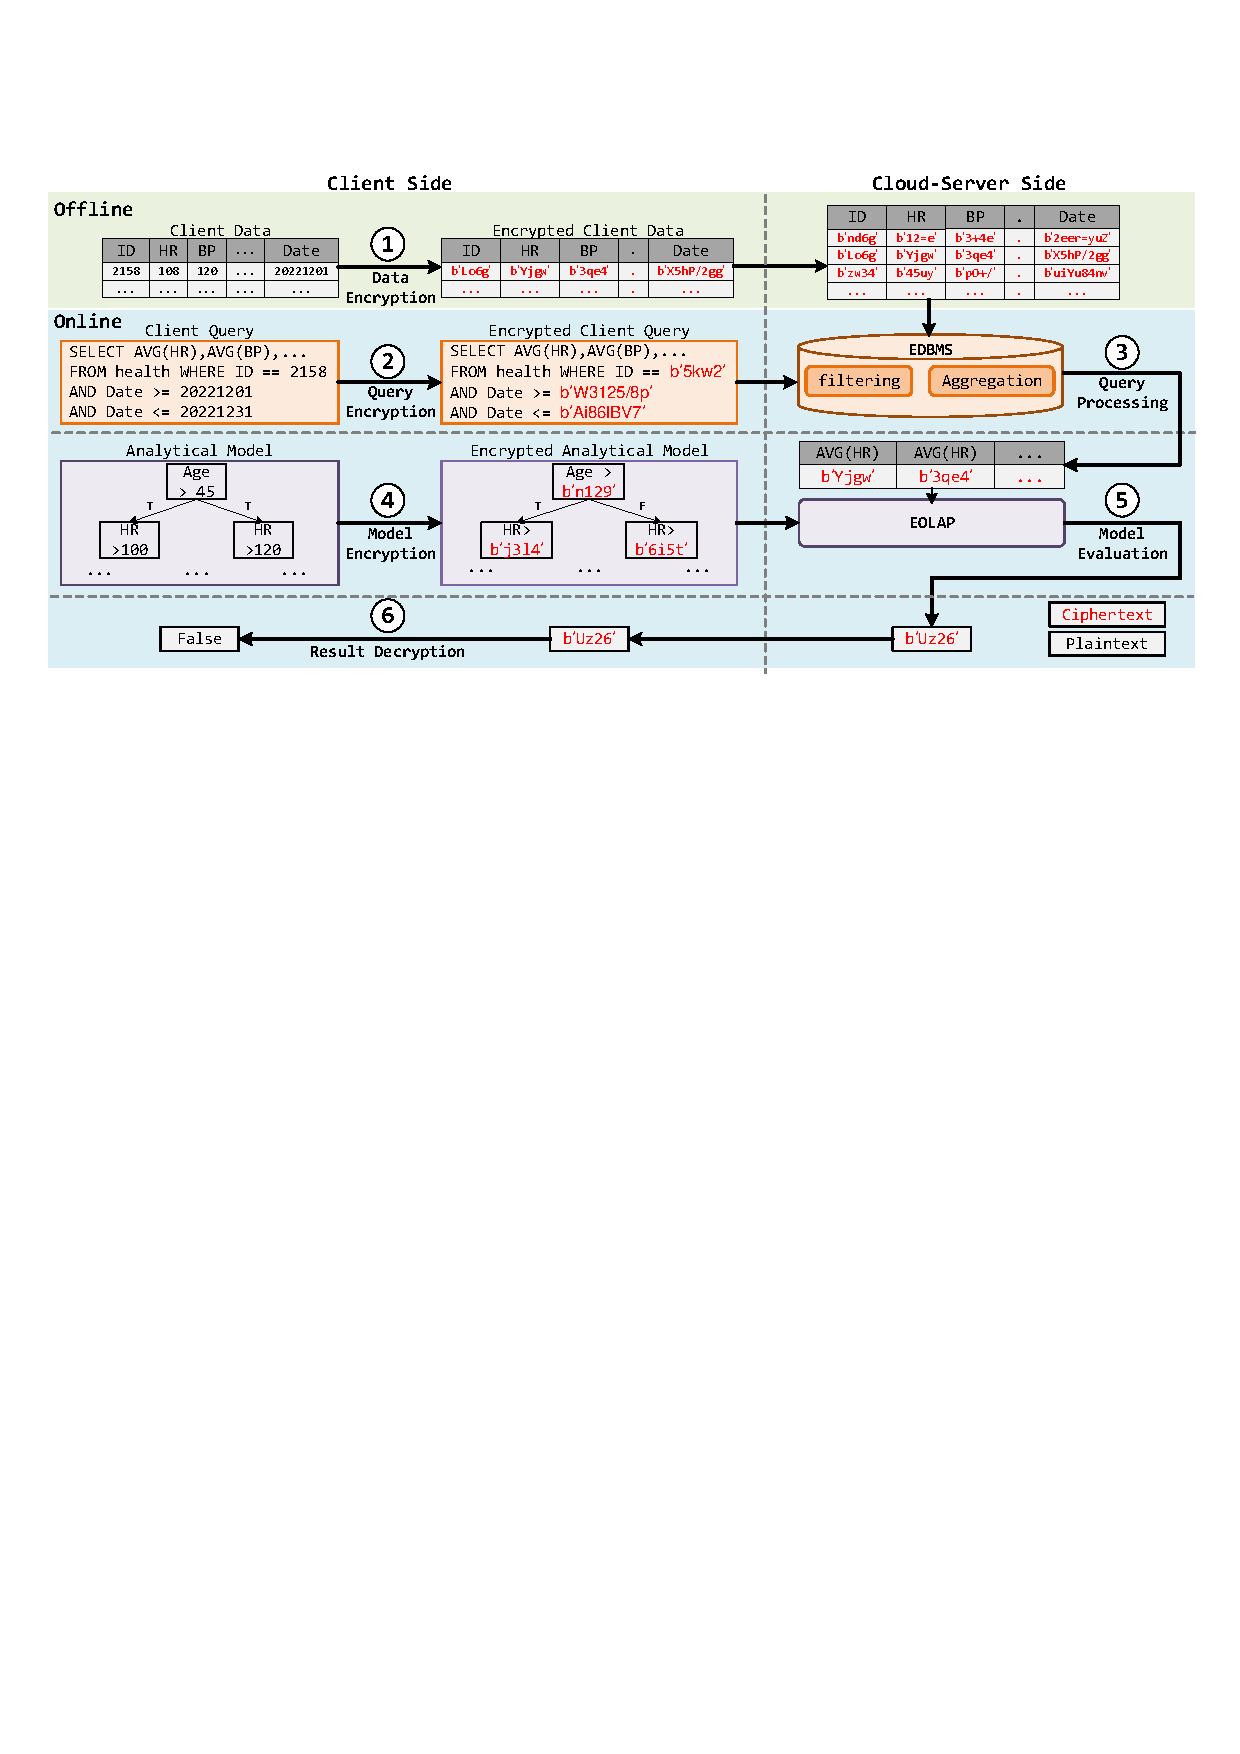
\includegraphics[width=\linewidth]{figure/overview.pdf}
%    \end{center}
%     \vspace{-0.5em}
%       \caption{A plaintext illustration in \cref{algo: 2kHMSB}. 
%       Each rectangle represents a decrypted plaintext while the left is 
%       the most significant bit.
%       The blue-colored region is the bits occupied by the message, 
%       the red-colored field is the bits filled with noise, 
%       and the white part is the bits set to zero.} 
%    \label{fig:overview}
%    \vspace{-0.5em}
% \end{figure*}





\subsection{Threat Model and Security} \label{overview:threat_model}
{\bf{Threat Model}}: Our security goal is to protect the privacy of 
client's $\mathcal{C}$ database $\mathcal{D}$ from the server $\mathcal{S}$.
Our threat model are similar to previous works\cite{heda, sortinghat, sagma}. 
To be more precise, we primarily consider a classic semi-honest model,
also known as an honest-but-curious adversary.
Here, the $\mathcal{C}$ encrypts the private $\mathcal{D}$
using FHE and outsources to the $\mathcal{S}$. 
The $\mathcal{S}$ honestly follows the \NAME workflow and
executes the queries or models on the $\mathcal{D}$, but acts as 
a probabilistic polynomial time adversary and perform the computation to try
learn as much as possible from the data provided by $\mathcal{C}$.
The specific availability of data to the server is as follows, we 
use $\mathcal{T}$ to denote the table, $\mathcal{Q}$ to represent the 
query and $\mathcal{M}$ as the analytical model.

\noindent {\bf{Public Data}}: The public information accessible to the 
server or attacker in \NAME is: 
\begin{itemize}
    \item The scheme of the database, that is, 
    the number of tables in $\mathcal{D}$
    $\lvert \mathcal{D} \rvert _{\mathcal{T}}$, 
    for each $\mathcal{T}$, 
    the label of the table and attributes, 
    the number of rows $\lvert \mathcal{T} \rvert _{r}$, 
    the number of columns $\lvert \mathcal{T} \rvert _{c}$.
    \item The structure of the query, i.e., 
    the number of filtering predicates
    $\lvert \mathcal{Q} \rvert $,
    the label of each predicate, 
    the type of each predicates(equality and inequality),
    the aggregation function and the attributes being aggregated. 
    \item The circuit of the analytical model,
    including the number of weight $\lvert \mathcal{M} \rvert$.
\end{itemize}

\noindent {\bf{Private Data}}: The private data that is unavailable to the 
public is: 
\begin{itemize}
    \item The domain value of the database, i.e.,  
    for each $\mathcal{T}$, 
    the value in certain rows and columns 
    $\mathcal{T}_{i, j}$, 
    for $i \in \lvert \mathcal{T} \rvert _{r}$
    for $j \in \lvert \mathcal{T} \rvert _{c}$.
    \item The predicate value of the query
    $\mathcal{Q}_{i}$, for $i \in \lvert \mathcal{Q} \rvert$. 
    \item The weight value of the analytical model 
    $\mathcal{M}_{j}$, for $j \in \lvert \mathcal{M} \rvert$.
\end{itemize}

{\bf{Security of \NAME}}: Since the private values are encrypted based 
on FHE, the security of \NAME could be directly 
reduced to the security of the FHE ciphertexts.
Traditional FHE schemes, such as B/FV, CKKS, and TFHE, 
all guarantee security under chosen plaintext attacks, 
which translates to a semi-honest security 
on the privacy of the client's private data. 
Assuming the circular security of the underlying FHE schemes, 
switching between different ciphertext formats preserves 
the overall semi-honest security of the protocol.
Since we utilize different FHE schemes in \NAME, 
we emphasize that the parameters of all 
FHE primitives need to be jointly 
adjusted to achieve the same level of security. 
Note that \NAME not only protects the filter values,
but also the selected entries 
as well as the number of selected entries 
during the querying process.
This protects access patterns as well as volume leakage in \NAME
and defends against a lot of leakage-abuse attacks\cite{...}.
However, like most FHE applications, 
the circuit privacy is out of the scope of this work.  

% \subsection{Key Ideas} \label{overview:key_ideas}

\begin{algorithm}[t!]
    % \tiny
    \caption{Homomorphic Query Evaluation Algorithm}
    \label{algo: query_evaluation}
    \SetKwInOut{Input}{Input}\SetKwInOut{Output}{Output}\SetKwInOut{Return}{Return}
    \SetKwComment{Comment}{$\triangleright$\ }{}
    \Input{Encrypted table $\mathcal{CT}=
    (ct_{1}, ct_{2}, ... , ct_{\lvert \mathcal{T} \rvert_{c}})$, 
    Encrypted Query $\mathcal{CQ}=
    (cp_{1}, cp_{2}, ... ,cp_{\lvert \mathcal{Q} \rvert}, B, G)$.
    Notations defined in \cref{pre: he_db}}
    \Output{A set of (R)LWE cipher $\mathcal{CR}
     = (cr_1, cr_2, ..., cr_{\lvert G \rvert})$.}
     Set $fl_{0,j} = {\rm LWE}(1)$ 
     for $j \in (1,2,...,\lvert \mathcal{T} \rvert_{r})$ and $b_0 = AND$\\
    \For{$i = 1$ \KwTo $\lvert \mathcal{Q} \rvert$}
    {
        $d = cp(a)_i$ \tcp*{Attribute index of $cp_i$} \\
        $op = cp(o)_i$ \tcp*{Operator of $cp_i$} \\
        $\mathbf{ct_d} = \texttt{SampleExtract}(ct_{d})$ 
        \tcp*{$\lvert \mathcal{T} \rvert_{r}$ LWEs}\\
        $\mathbf{cp_i} = \texttt{SampleExtract}(cp_{i})$ \Comment*[r]{$i-th$ index}\\
        \For{$j = 1$ \KwTo $\lvert \mathcal{T} \rvert_{r}$}
        {
            $comp_{i,j} = \texttt{HomComp}
            (\mathbf{ct_d}[j], \mathbf{cp_i}[j],op)$ \\
            $fl_{i,j} = \texttt{HomGate}(fl_{i-1, j}, comp_{i,j}, b_{i-1})$ \\
        }
    }
    $fl = \texttt{LWEsPack}(fl_{\abs{Q}, 1},fl_{\abs{Q}, 2}...,fl_{\abs{Q}, \abs{T}})$\tcp*[f]{A RLWE} \\
    \For{$i = 1$ \KwTo $\lvert G \rvert$}
    {
        $d = g(a)_i$ \\
        $f_i = g(f)_i$ \\
        \eIf{$g_i$ is support coeffcient}
        {
            $cr_i = \texttt{Homfun}(fl, ct_d, f_i, \texttt{Coeff})$ \\
        }
        {
            $\hat{ct_d} = \texttt{SlotToCoeff}(ct_d)$ \\
            $\hat{fl} = \texttt{SlotToCoeff}(fl)$ \\
            $cr_i = \texttt{Homfun}(\hat{fl}, \hat{ct_d}, f_i, \texttt{Slot})$ \\
        }
    }
    \Return{$\mathcal{CR}
     = (cr_1, cr_2, ..., cr_{\abs{G}})$}
\end{algorithm}



